% Options for packages loaded elsewhere
\PassOptionsToPackage{unicode}{hyperref}
\PassOptionsToPackage{hyphens}{url}
\PassOptionsToPackage{dvipsnames,svgnames,x11names}{xcolor}
%
\documentclass[
  12pt,
]{article}

\usepackage{amsmath,amssymb}
\usepackage{setspace}
\usepackage{iftex}
\ifPDFTeX
  \usepackage[T1]{fontenc}
  \usepackage[utf8]{inputenc}
  \usepackage{textcomp} % provide euro and other symbols
\else % if luatex or xetex
  \usepackage{unicode-math}
  \defaultfontfeatures{Scale=MatchLowercase}
  \defaultfontfeatures[\rmfamily]{Ligatures=TeX,Scale=1}
\fi
\usepackage[]{newtxsf}
\ifPDFTeX\else  
    % xetex/luatex font selection
\fi
% Use upquote if available, for straight quotes in verbatim environments
\IfFileExists{upquote.sty}{\usepackage{upquote}}{}
\IfFileExists{microtype.sty}{% use microtype if available
  \usepackage[]{microtype}
  \UseMicrotypeSet[protrusion]{basicmath} % disable protrusion for tt fonts
}{}
\usepackage{xcolor}
\usepackage[top=31.8mm,bottom=31.8mm,right=24.5mm,left=24.5mm]{geometry}
\setlength{\emergencystretch}{3em} % prevent overfull lines
\setcounter{secnumdepth}{5}
% Make \paragraph and \subparagraph free-standing
\makeatletter
\ifx\paragraph\undefined\else
  \let\oldparagraph\paragraph
  \renewcommand{\paragraph}{
    \@ifstar
      \xxxParagraphStar
      \xxxParagraphNoStar
  }
  \newcommand{\xxxParagraphStar}[1]{\oldparagraph*{#1}\mbox{}}
  \newcommand{\xxxParagraphNoStar}[1]{\oldparagraph{#1}\mbox{}}
\fi
\ifx\subparagraph\undefined\else
  \let\oldsubparagraph\subparagraph
  \renewcommand{\subparagraph}{
    \@ifstar
      \xxxSubParagraphStar
      \xxxSubParagraphNoStar
  }
  \newcommand{\xxxSubParagraphStar}[1]{\oldsubparagraph*{#1}\mbox{}}
  \newcommand{\xxxSubParagraphNoStar}[1]{\oldsubparagraph{#1}\mbox{}}
\fi
\makeatother
\usepackage{color}
\usepackage{fancyvrb}
\newcommand{\VerbBar}{|}
\newcommand{\VERB}{\Verb[commandchars=\\\{\}]}
\DefineVerbatimEnvironment{Highlighting}{Verbatim}{commandchars=\\\{\}}
% Add ',fontsize=\small' for more characters per line
\usepackage{framed}
\definecolor{shadecolor}{RGB}{241,243,245}
\newenvironment{Shaded}{\begin{snugshade}}{\end{snugshade}}
\newcommand{\AlertTok}[1]{\textcolor[rgb]{0.68,0.00,0.00}{#1}}
\newcommand{\AnnotationTok}[1]{\textcolor[rgb]{0.37,0.37,0.37}{#1}}
\newcommand{\AttributeTok}[1]{\textcolor[rgb]{0.40,0.45,0.13}{#1}}
\newcommand{\BaseNTok}[1]{\textcolor[rgb]{0.68,0.00,0.00}{#1}}
\newcommand{\BuiltInTok}[1]{\textcolor[rgb]{0.00,0.23,0.31}{#1}}
\newcommand{\CharTok}[1]{\textcolor[rgb]{0.13,0.47,0.30}{#1}}
\newcommand{\CommentTok}[1]{\textcolor[rgb]{0.37,0.37,0.37}{#1}}
\newcommand{\CommentVarTok}[1]{\textcolor[rgb]{0.37,0.37,0.37}{\textit{#1}}}
\newcommand{\ConstantTok}[1]{\textcolor[rgb]{0.56,0.35,0.01}{#1}}
\newcommand{\ControlFlowTok}[1]{\textcolor[rgb]{0.00,0.23,0.31}{\textbf{#1}}}
\newcommand{\DataTypeTok}[1]{\textcolor[rgb]{0.68,0.00,0.00}{#1}}
\newcommand{\DecValTok}[1]{\textcolor[rgb]{0.68,0.00,0.00}{#1}}
\newcommand{\DocumentationTok}[1]{\textcolor[rgb]{0.37,0.37,0.37}{\textit{#1}}}
\newcommand{\ErrorTok}[1]{\textcolor[rgb]{0.68,0.00,0.00}{#1}}
\newcommand{\ExtensionTok}[1]{\textcolor[rgb]{0.00,0.23,0.31}{#1}}
\newcommand{\FloatTok}[1]{\textcolor[rgb]{0.68,0.00,0.00}{#1}}
\newcommand{\FunctionTok}[1]{\textcolor[rgb]{0.28,0.35,0.67}{#1}}
\newcommand{\ImportTok}[1]{\textcolor[rgb]{0.00,0.46,0.62}{#1}}
\newcommand{\InformationTok}[1]{\textcolor[rgb]{0.37,0.37,0.37}{#1}}
\newcommand{\KeywordTok}[1]{\textcolor[rgb]{0.00,0.23,0.31}{\textbf{#1}}}
\newcommand{\NormalTok}[1]{\textcolor[rgb]{0.00,0.23,0.31}{#1}}
\newcommand{\OperatorTok}[1]{\textcolor[rgb]{0.37,0.37,0.37}{#1}}
\newcommand{\OtherTok}[1]{\textcolor[rgb]{0.00,0.23,0.31}{#1}}
\newcommand{\PreprocessorTok}[1]{\textcolor[rgb]{0.68,0.00,0.00}{#1}}
\newcommand{\RegionMarkerTok}[1]{\textcolor[rgb]{0.00,0.23,0.31}{#1}}
\newcommand{\SpecialCharTok}[1]{\textcolor[rgb]{0.37,0.37,0.37}{#1}}
\newcommand{\SpecialStringTok}[1]{\textcolor[rgb]{0.13,0.47,0.30}{#1}}
\newcommand{\StringTok}[1]{\textcolor[rgb]{0.13,0.47,0.30}{#1}}
\newcommand{\VariableTok}[1]{\textcolor[rgb]{0.07,0.07,0.07}{#1}}
\newcommand{\VerbatimStringTok}[1]{\textcolor[rgb]{0.13,0.47,0.30}{#1}}
\newcommand{\WarningTok}[1]{\textcolor[rgb]{0.37,0.37,0.37}{\textit{#1}}}

\providecommand{\tightlist}{%
  \setlength{\itemsep}{0pt}\setlength{\parskip}{0pt}}\usepackage{longtable,booktabs,array}
\usepackage{calc} % for calculating minipage widths
% Correct order of tables after \paragraph or \subparagraph
\usepackage{etoolbox}
\makeatletter
\patchcmd\longtable{\par}{\if@noskipsec\mbox{}\fi\par}{}{}
\makeatother
% Allow footnotes in longtable head/foot
\IfFileExists{footnotehyper.sty}{\usepackage{footnotehyper}}{\usepackage{footnote}}
\makesavenoteenv{longtable}
\usepackage{graphicx}
\makeatletter
\newsavebox\pandoc@box
\newcommand*\pandocbounded[1]{% scales image to fit in text height/width
  \sbox\pandoc@box{#1}%
  \Gscale@div\@tempa{\textheight}{\dimexpr\ht\pandoc@box+\dp\pandoc@box\relax}%
  \Gscale@div\@tempb{\linewidth}{\wd\pandoc@box}%
  \ifdim\@tempb\p@<\@tempa\p@\let\@tempa\@tempb\fi% select the smaller of both
  \ifdim\@tempa\p@<\p@\scalebox{\@tempa}{\usebox\pandoc@box}%
  \else\usebox{\pandoc@box}%
  \fi%
}
% Set default figure placement to htbp
\def\fps@figure{htbp}
\makeatother
% definitions for citeproc citations
\NewDocumentCommand\citeproctext{}{}
\NewDocumentCommand\citeproc{mm}{%
  \begingroup\def\citeproctext{#2}\cite{#1}\endgroup}
\makeatletter
 % allow citations to break across lines
 \let\@cite@ofmt\@firstofone
 % avoid brackets around text for \cite:
 \def\@biblabel#1{}
 \def\@cite#1#2{{#1\if@tempswa , #2\fi}}
\makeatother
\newlength{\cslhangindent}
\setlength{\cslhangindent}{1.5em}
\newlength{\csllabelwidth}
\setlength{\csllabelwidth}{3em}
\newenvironment{CSLReferences}[2] % #1 hanging-indent, #2 entry-spacing
 {\begin{list}{}{%
  \setlength{\itemindent}{0pt}
  \setlength{\leftmargin}{0pt}
  \setlength{\parsep}{0pt}
  % turn on hanging indent if param 1 is 1
  \ifodd #1
   \setlength{\leftmargin}{\cslhangindent}
   \setlength{\itemindent}{-1\cslhangindent}
  \fi
  % set entry spacing
  \setlength{\itemsep}{#2\baselineskip}}}
 {\end{list}}
\usepackage{calc}
\newcommand{\CSLBlock}[1]{\hfill\break\parbox[t]{\linewidth}{\strut\ignorespaces#1\strut}}
\newcommand{\CSLLeftMargin}[1]{\parbox[t]{\csllabelwidth}{\strut#1\strut}}
\newcommand{\CSLRightInline}[1]{\parbox[t]{\linewidth - \csllabelwidth}{\strut#1\strut}}
\newcommand{\CSLIndent}[1]{\hspace{\cslhangindent}#1}

% Appele dans "include-in-header", donc n'a pas acces aux variables du YAML du document ex: 'title'
% Peut-etre demenager tout ca dans 'before-body.tex'???

\usepackage{graphicx}
\graphicspath{ {./_images/} }

\usepackage[skip=10pt plus1pt, indent=40pt]{parskip}
\makeatletter
\@ifpackageloaded{caption}{}{\usepackage{caption}}
\AtBeginDocument{%
\ifdefined\contentsname
  \renewcommand*\contentsname{Table of contents}
\else
  \newcommand\contentsname{Table of contents}
\fi
\ifdefined\listfigurename
  \renewcommand*\listfigurename{List of Figures}
\else
  \newcommand\listfigurename{List of Figures}
\fi
\ifdefined\listtablename
  \renewcommand*\listtablename{List of Tables}
\else
  \newcommand\listtablename{List of Tables}
\fi
\ifdefined\figurename
  \renewcommand*\figurename{Figure}
\else
  \newcommand\figurename{Figure}
\fi
\ifdefined\tablename
  \renewcommand*\tablename{Table}
\else
  \newcommand\tablename{Table}
\fi
}
\@ifpackageloaded{float}{}{\usepackage{float}}
\floatstyle{ruled}
\@ifundefined{c@chapter}{\newfloat{codelisting}{h}{lop}}{\newfloat{codelisting}{h}{lop}[chapter]}
\floatname{codelisting}{Listing}
\newcommand*\listoflistings{\listof{codelisting}{List of Listings}}
\makeatother
\makeatletter
\makeatother
\makeatletter
\@ifpackageloaded{caption}{}{\usepackage{caption}}
\@ifpackageloaded{subcaption}{}{\usepackage{subcaption}}
\makeatother


% Configuration de l'entête
\usepackage{fancyhdr}
\pagestyle{fancy}
\fancyhead[L]{{Rapport de session}}
\fancyfoot[C]{\thepage}

% Configuration du bas de page
  \fancyfoot[L]{\textcopyright \ Benjamin 2025}

\usepackage{bookmark}

\IfFileExists{xurl.sty}{\usepackage{xurl}}{} % add URL line breaks if available
\urlstyle{same} % disable monospaced font for URLs
\hypersetup{
  pdftitle={Rapport de session},
  pdfauthor={Benjamin},
  colorlinks=true,
  linkcolor={blue},
  filecolor={Maroon},
  citecolor={Blue},
  urlcolor={Blue},
  pdfcreator={LaTeX via pandoc}}


\title{Rapport de session}
\author{Benjamin}
\date{2025-03-20}

\begin{document}

  
  \begin{titlepage} 
      \centering
      {\large DEPARTEMENT DES SCIENCES DU BOIS ET DE LA FORET \\}
      {\large FACULTE DE FORESTERIE, DE GEOGRAPHIE ET DE GEOMATIQUE \\}
      {\large UNIVERSITE LAVAL \\}
       %{
\includegraphics[width=1.5cm]{logo-quarto} \\}
          
\includegraphics[width=1.5cm]{logo-quarto} \\
      
      \vfill %\vspace{2cm}
      {\Huge\bfseries\underline {Rapport de session} \par}
      \vfill %\vspace{2cm}
              \ifnum 1 = 1
              {\Large Auteur : \\}
          \else
              {\Large Auteurs : \\}
          \fi
          {\large {Benjamin}}
          \vfill
      {\Large À l'intention de: \\ {Albert Einstein}}
      \vfill
      {\large Quebec, {2025-03-20}}
  \end{titlepage}
\pagenumbering{roman}

  \renewcommand{\abstractname}{\section*{Résumé}\label{ruxe9sumuxe9}}
  \begin{abstract}
    \begin{center}
      \addcontentsline{toc}{section}{Résumé}
      Lorem ipsum dolor sit amet, consectetuer adipiscing elit. Etiam
      lobortisfacilisis sem. Nullam nec mi et neque pharetra
      sollicitudin. Praesent imperdietmi nec ante. Donec ullamcorper,
      felis non sodales\ldots{}
    \end{center}
    {\newpage}
  \end{abstract}

  \begin{center}
    \section*{Remerciements}\label{remerciement}
    \addcontentsline{toc}{section}{Remerciements}
    Lorem ipsum dolor sit amet, consectetuer adipiscing elit. Etiam
    lobortisfacilisis sem. Nullam nec mi et neque pharetra sollicitudin.
    Praesent imperdietmi nec ante. Donec ullamcorper, felis non
    sodales\ldots{}
  \end{center}
  {\newpage}


%%%% la pagination a été déplacé dans le "before-body.tex" %%%%
% \pagenumbering{roman}

\renewcommand*\contentsname{Table des matieres}
\tableofcontents

\newpage

\renewcommand\listfigurename{Liste des figures}
\listoffigures

\renewcommand\listtablename{Liste des tableaux}
\listoftables

\newpage

\pagenumbering{arabic}
\setcounter{page}{1}
\renewcommand\tablename{Tableau}
\renewcommand\figurename{Figure}
\setstretch{1.5}
\section{Introduction}\label{introduction}

Bonjour dans ce texte, nous allons parler du dispositif expérimental
établis par Steve Bédard (2022) dans la forêt expérimentale de
Duchesnay. En 2020, le gouvernement québécois annonce avoir atteint 17\%
de son territoire sous le status d'aire protégée (Radio-Canada, 2020).
En 2022, lors du cadre mondiale de la biodiversité Kumming-Montréal,
l'un des objectifs auxquels le Canada s'est engagé à respecter est la
protection de 30\% de ses écosystèmes terrestres, marin, d'eaux
intérieures et côtiers d'ici 2030 (ONU, 2022).

Afin de rencontrer la cible de 30\% d'aire protégée sur territoire, le
Québec a apporté des modification à la Loi sur la conservation du
patrimoine naturel (LCPN) en 2021. Cette modification apportera une
accélération du processus de création d'aire protégée, d'inclure
davantage les citoyens dans la création et la gestion d'aire protégée et
finalement de diversifier les types de mesures de conservation (MELCCFP,
2025). Dans la région de Portneuf, un projet reflètant les grands
objectifs de la modernisation de la LCPN a été entrepris par le Conseil
de Nation Huron-Wendat depuis 2010 (Bérubé, 2021). Ce projet d'aire
protégée à utilisation durable serait un outil incontournable pour la
mise en oeuvre de la protection de 30\% du territoire.

Le dispoisitif est composé de quatre blocs, chacun composé de cinq
unités expérimentals (Bédard, Raymond, and DeBlois 2022). Afin de
rencontrer la cible de 30\% d'aire protégée sur territoire, le Québec a
apporté des modification à la Loi sur la conservation du patrimoine
naturel (LCPN) en 2021. Cette modification apportera une accélération du
processus de création d'aire protégée, d'inclure davantage les citoyens
dans la création et la gestion d'aire protégée et finalement de
diversifier les types de mesures de conservation (MELCCFP, 2025). Dans
la région de Portneuf, un projet reflètant les grands objectifs de la
modernisation de la LCPN a été entrepris par le Conseil de Nation
Huron-Wendat depuis 2010 (Bérubé, 2021). Ce projet d'aire protégée à
utilisation durable serait un outil incontournable pour la mise en
oeuvre de la protection de 30\% du territoire.

\section{Méthode}\label{muxe9thode}

\section{Résultat}\label{ruxe9sultat}

Afin de rencontrer la cible de 30\% d'aire protégée sur territoire, le
Québec a apporté des modification à la Loi sur la conservation du
patrimoine naturel (LCPN) en 2021. Cette modification apportera une
accélération du processus de création d'aire protégée, d'inclure
davantage les citoyens dans la création et la gestion d'aire protégée et
finalement de diversifier les types de mesures de conservation (MELCCFP,
2025). Dans la région de Portneuf, un projet reflètant les grands
objectifs de la modernisation de la LCPN a été entrepris par le Conseil
de Nation Huron-Wendat depuis 2010 (Bérubé, 2021). Ce projet d'aire
protégée à utilisation durable serait un outil incontournable pour la
mise en oeuvre de la protection de 30\% du territoire.

\subsection{Exemple de tableau}\label{exemple-de-tableau}

\begin{longtable}[]{@{}lr@{}}
\caption{Prix unitaire des fruits}\tabularnewline
\toprule\noalign{}
\textbf{fruit} & \textbf{prix (\$/lbs)} \\
\midrule\noalign{}
\endfirsthead
\toprule\noalign{}
\textbf{fruit} & \textbf{prix (\$/lbs)} \\
\midrule\noalign{}
\endhead
\bottomrule\noalign{}
\endlastfoot
banane & 2.05 \\
pomme & 0.75 \\
fraise & 3.00 \\
\end{longtable}

\subsection{Exemple de figure}\label{exemple-de-figure}

\begin{Shaded}
\begin{Highlighting}[]
\ImportTok{import}\NormalTok{ numpy }\ImportTok{as}\NormalTok{ np}
\ImportTok{import}\NormalTok{ matplotlib.pyplot }\ImportTok{as}\NormalTok{ plt}

\NormalTok{r }\OperatorTok{=}\NormalTok{ np.arange(}\DecValTok{0}\NormalTok{, }\DecValTok{2}\NormalTok{, }\FloatTok{0.01}\NormalTok{)}
\NormalTok{theta }\OperatorTok{=} \DecValTok{2} \OperatorTok{*}\NormalTok{ np.pi }\OperatorTok{*}\NormalTok{ r}
\NormalTok{fig, ax }\OperatorTok{=}\NormalTok{ plt.subplots(}
\NormalTok{  subplot\_kw }\OperatorTok{=}\NormalTok{ \{}\StringTok{\textquotesingle{}projection\textquotesingle{}}\NormalTok{: }\StringTok{\textquotesingle{}polar\textquotesingle{}}\NormalTok{\} }
\NormalTok{)}
\NormalTok{ax.plot(theta, r)}
\NormalTok{ax.set\_rticks([}\FloatTok{0.5}\NormalTok{, }\DecValTok{1}\NormalTok{, }\FloatTok{1.5}\NormalTok{, }\DecValTok{2}\NormalTok{])}
\NormalTok{ax.grid(}\VariableTok{True}\NormalTok{)}
\NormalTok{plt.show()}
\end{Highlighting}
\end{Shaded}

\begin{figure}[H]

\centering{

\pandocbounded{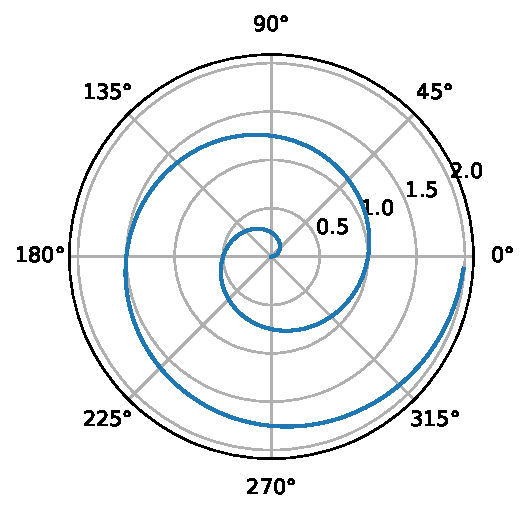
\includegraphics[keepaspectratio]{exemple_VSCode_files/figure-pdf/fig-polar-output-1.pdf}}

}

\caption{\label{fig-polar}A line plot on a polar axis}

\end{figure}%

\section{Discussion}\label{discussion}

\section{Conclusion}\label{conclusion}

\newpage{}

\section*{Bibliographie}\label{bibliographie}
\addcontentsline{toc}{section}{Bibliographie}

\phantomsection\label{refs}
\begin{CSLReferences}{1}{0}
\bibitem[\citeproctext]{ref-bedard_northern_2022}
Bédard, Steve, Patricia Raymond, and Josianne DeBlois. 2022. {``Northern
Hardwood Regeneration Dynamics 10 Years After Irregular Shelterwood and
Mechanical Control of Understory American Beech.''} \emph{Forest Ecology
and Management} 511 (May): 120142.
\url{https://doi.org/10.1016/j.foreco.2022.120142}.

\end{CSLReferences}




\end{document}
